% This is a template for our talks
\documentclass[12pt,english,dvipsnames]{beamer}

\usepackage{sosy-beamer}
% \usepackage[scaled=0.8]{beramono}
\usepackage{amssymb,amsmath,mathtools}
\usepackage{tabto}
\usepackage{tikz}
\usetikzlibrary{cd}

\newcommand{\red}[1]{{\color{red}#1}}
\newcommand{\blue}[1]{{\color{blue}#1}}
\newcommand{\green}[1]{{\color{cpacheckergreen}#1}}
\newcommand{\Yes}{\green{\cmark}}
\newcommand{\No}{\red{\xmark}}

\newcommand{\code}[1]{\text{\upshape\ttfamily#1}}
\newcommand{\graycode}[1]{\code{\color{darkgray}#1}}
\newcommand{\low}{\code{low}}
\newcommand{\high}{\code{high}}
\newcommand{\id}{\mathit{id}}
\newcommand{\fp}{\mathit{fp}}
\newcommand{\blob}{\mathit{pk}}
\newcommand{\fingerprint}{\code{fingerprint}}
\newcommand{\haslabel}{\mathbin{\dblcolon}}
\newcommand{\Key}[2]{\code{Key}(#1,\,#2)}

\newcommand{\hoare}[3]{\{ #1 \}~~#2~~\{ #3 \}}
\newcommand{\loweq}{\equiv_\low}

\newcommand{\True}{\texttt{true}}
\newcommand{\False}{\texttt{false}}

\author{Gidon Ernst \and Lukas Rieger}
\title{Information Flow Testing\\of a PGP Keyserver}
\subtitle{VerifyThis long-term challenge 2020}

\institute[LMU Munich]{LMU Munich, Germany}

\date{}

\begin{document}

\begin{frame}
    \centering
    {\Large \inserttitle}
    \bigskip

    {       \insertsubtitle}

    \bigskip

    \begin{minipage}[b]{2.5cm}
      \centering
    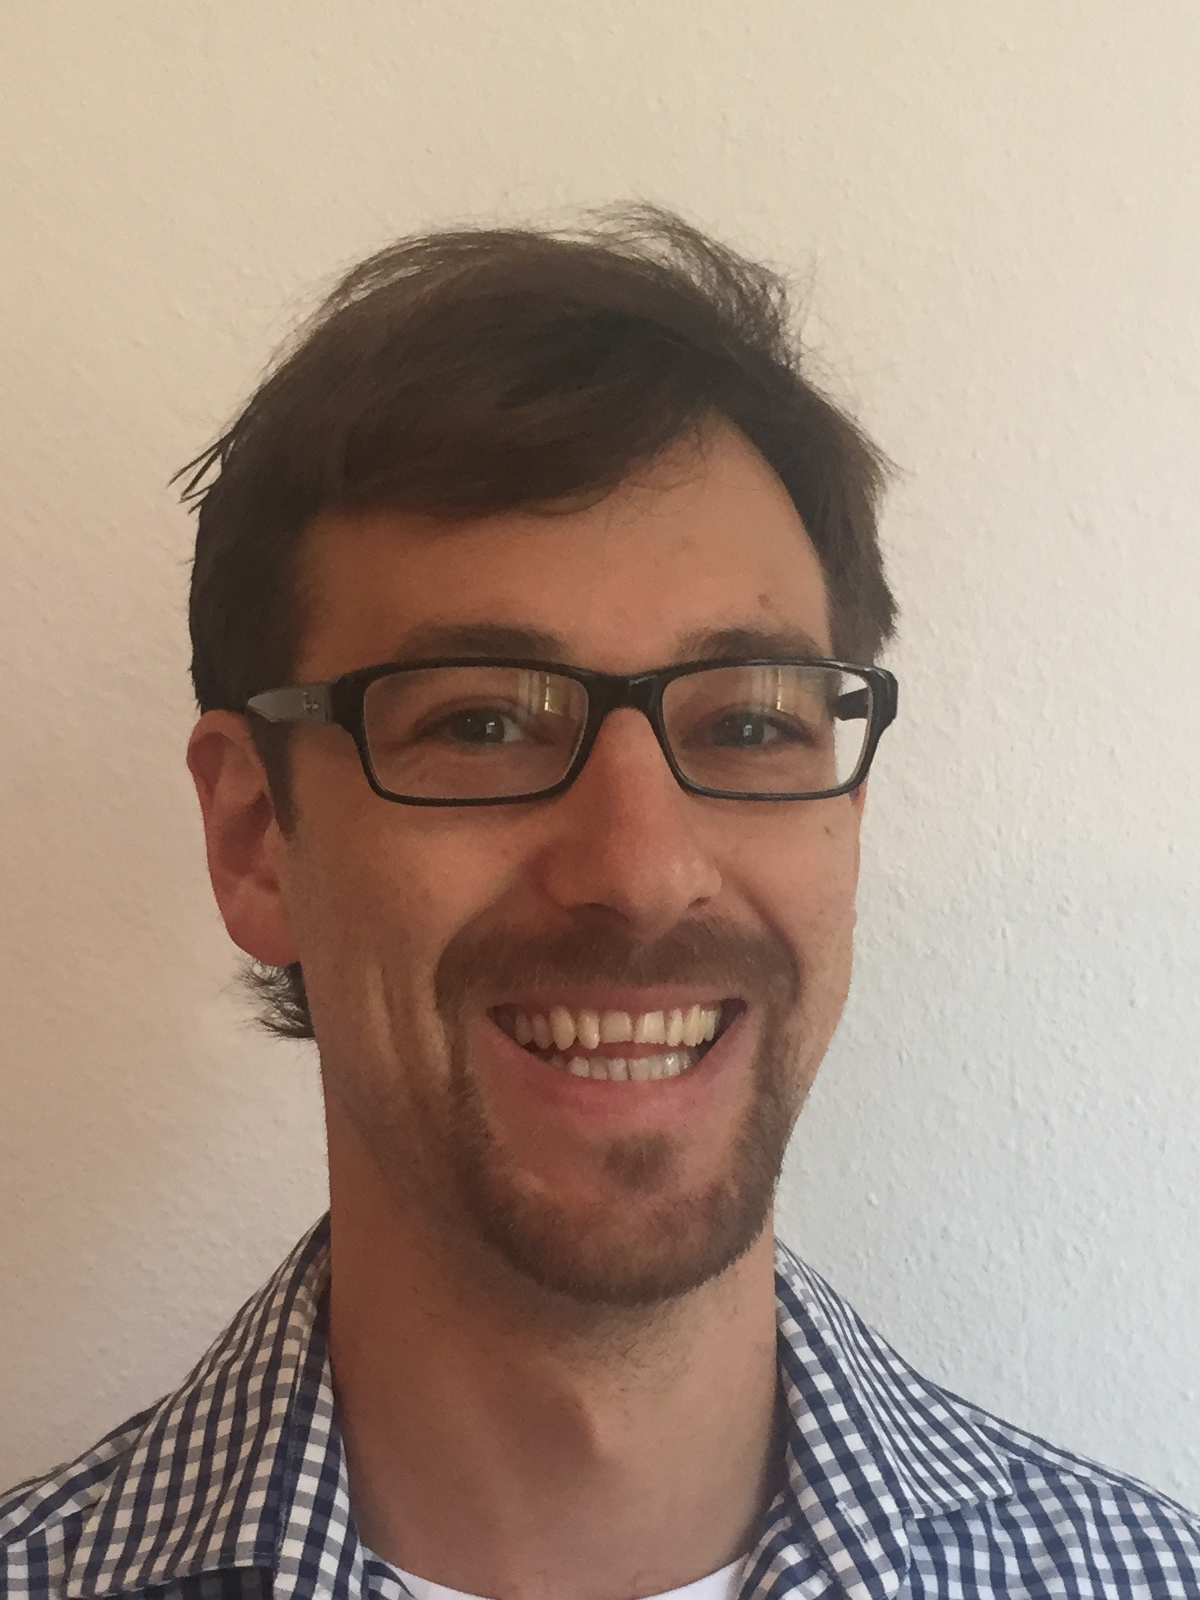
\includegraphics[height=2.5cm]{images/gernst} \\
    Gidon Ernst
    \end{minipage}
    \quad
    \begin{minipage}[b]{2.5cm}
      \centering
    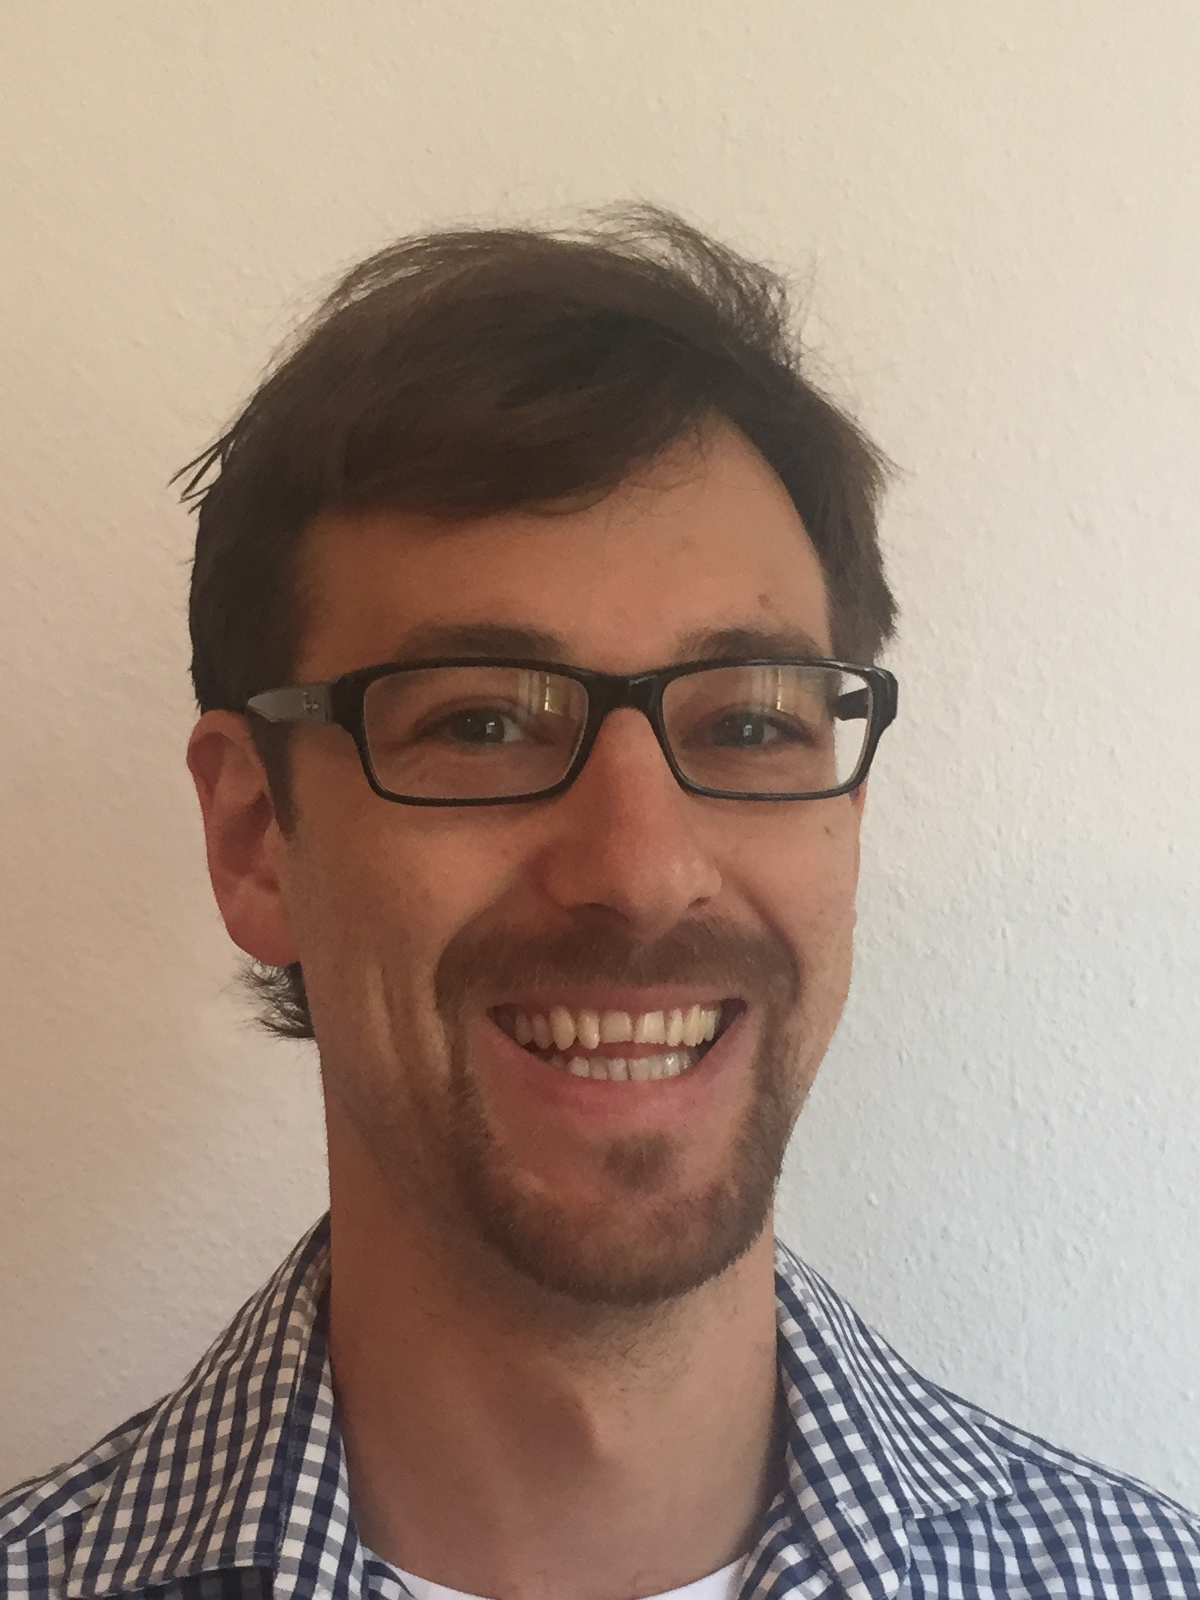
\includegraphics[height=2.5cm]{images/gernst} \\
    Lukas Rieger
    \end{minipage}
    \quad
    \begin{minipage}[b]{3cm}
      \centering
    \resizebox{!}{1cm}{% Created with inkscape
\documentclass{standalone}
\usepackage{../sosy-beamer}

\begin{document}

\begin{tikzpicture}[y=0.80pt, x=0.80pt, yscale=-1.000000, xscale=1.000000, inner sep=0pt, outer sep=0pt]
\begin{scope}
  \begin{scope}[fill=black]
  \end{scope}
  \begin{scope}[fill=black]
  \end{scope}
  \begin{scope}[fill=black]
  \end{scope}
  % Inner border
  \path[draw=unigrey,fill=sosyblue,miter limit=4.00,nonzero rule,line
    width=1.680pt] (115.4930,729.8772) -- (292.9577,729.8772) .. controls
    (309.3159,729.8772) and (322.4850,743.0464) .. (322.4850,759.4045) .. controls
    (322.4850,775.7626) and (309.3159,788.9317) .. (292.9577,788.9317) --
    (115.4930,788.9317) .. controls (99.1349,788.9317) and (85.9657,775.7626) ..
    (85.9657,759.4045) .. controls (85.9657,743.0464) and (99.1349,729.8772) ..
    (115.4930,729.8772) -- cycle;
  % "SoSy-Lab" lettering
  \begin{scope}[fill=black]
    \path[fill] (128.4041,765.7802) .. controls (128.4040,767.1708) and
      (128.1306,768.4521) .. (127.5837,769.6240) .. controls (127.0525,770.7958) and
      (126.2243,771.8115) .. (125.0994,772.6708) .. controls (123.9743,773.5146) and
      (122.5525,774.1786) .. (120.8337,774.6630) .. controls (119.1306,775.1318) and
      (117.1072,775.3661) .. (114.7634,775.3661) .. controls (110.6540,775.3661) and
      (107.4509,774.6474) .. (105.1541,773.2099) .. controls (102.8572,771.7724) and
      (101.3962,769.6943) .. (100.7712,766.9755) -- (105.1072,766.1083) .. controls
      (105.3259,766.9677) and (105.6619,767.7490) .. (106.1150,768.4521) .. controls
      (106.5681,769.1552) and (107.1775,769.7646) .. (107.9431,770.2802) .. controls
      (108.7244,770.7802) and (109.6853,771.1708) .. (110.8259,771.4521) .. controls
      (111.9665,771.7333) and (113.3337,771.8740) .. (114.9275,771.8740) .. controls
      (116.2556,771.8740) and (117.4743,771.7646) .. (118.5837,771.5458) .. controls
      (119.6931,771.3115) and (120.6462,770.9599) .. (121.4431,770.4911) .. controls
      (122.2400,770.0224) and (122.8572,769.4208) .. (123.2947,768.6865) .. controls
      (123.7478,767.9365) and (123.9743,767.0458) .. (123.9744,766.0146) .. controls
      (123.9743,764.9365) and (123.7243,764.0615) .. (123.2244,763.3896) .. controls
      (122.7400,762.7177) and (122.0525,762.1630) .. (121.1619,761.7255) .. controls
      (120.2712,761.2880) and (119.2087,760.9208) .. (117.9744,760.6240) .. controls
      (116.7400,760.3271) and (115.3728,760.0068) .. (113.8728,759.6630) .. controls
      (112.9509,759.4599) and (112.0212,759.2412) .. (111.0837,759.0068) .. controls
      (110.1619,758.7568) and (109.2712,758.4677) .. (108.4119,758.1396) .. controls
      (107.5681,757.7958) and (106.7712,757.3974) .. (106.0212,756.9443) .. controls
      (105.2712,756.4912) and (104.6228,755.9521) .. (104.0759,755.3271) .. controls
      (103.5290,754.6865) and (103.0994,753.9521) .. (102.7869,753.1240) .. controls
      (102.4744,752.2802) and (102.3181,751.3115) .. (102.3181,750.2177) .. controls
      (102.3181,748.6552) and (102.6306,747.3193) .. (103.2556,746.2099) .. controls
      (103.8962,745.0849) and (104.7790,744.1631) .. (105.9041,743.4443) .. controls
      (107.0290,742.7256) and (108.3572,742.2021) .. (109.8884,741.8740) .. controls
      (111.4197,741.5459) and (113.0759,741.3818) .. (114.8572,741.3818) .. controls
      (116.9040,741.3818) and (118.6540,741.5459) .. (120.1072,741.8740) .. controls
      (121.5603,742.1865) and (122.7868,742.6631) .. (123.7869,743.3037) .. controls
      (124.7868,743.9443) and (125.5837,744.7412) .. (126.1775,745.6943) .. controls
      (126.7868,746.6318) and (127.2712,747.7256) .. (127.6306,748.9755) --
      (123.2244,749.7490) .. controls (123.0056,748.9521) and (122.6853,748.2412) ..
      (122.2634,747.6162) .. controls (121.8572,746.9912) and (121.3181,746.4677) ..
      (120.6462,746.0458) .. controls (119.9743,745.6240) and (119.1540,745.3037) ..
      (118.1853,745.0849) .. controls (117.2322,744.8662) and (116.1072,744.7568) ..
      (114.8103,744.7568) .. controls (113.2790,744.7568) and (111.9900,744.8974) ..
      (110.9431,745.1787) .. controls (109.9119,745.4443) and (109.0759,745.8115) ..
      (108.4353,746.2802) .. controls (107.8103,746.7490) and (107.3572,747.3037) ..
      (107.0759,747.9443) .. controls (106.8103,748.5693) and (106.6775,749.2490) ..
      (106.6775,749.9833) .. controls (106.6775,750.9677) and (106.9197,751.7802) ..
      (107.4041,752.4208) .. controls (107.9040,753.0459) and (108.5759,753.5693) ..
      (109.4197,753.9912) .. controls (110.2634,754.4131) and (111.2400,754.7646) ..
      (112.3494,755.0458) .. controls (113.4587,755.3271) and (114.6384,755.6084) ..
      (115.8884,755.8896) .. controls (116.9040,756.1240) and (117.9118,756.3662) ..
      (118.9119,756.6162) .. controls (119.9275,756.8505) and (120.8962,757.1396) ..
      (121.8181,757.4833) .. controls (122.7400,757.8115) and (123.5993,758.2021) ..
      (124.3962,758.6552) .. controls (125.2087,759.1084) and (125.9118,759.6630) ..
      (126.5056,760.3193) .. controls (127.0993,760.9755) and (127.5603,761.7490) ..
      (127.8884,762.6396) .. controls (128.2321,763.5302) and (128.4040,764.5771) ..
      (128.4041,765.7802);
    \path[fill] (155.3337,762.1943) .. controls (155.3337,766.6318) and
      (154.3571,769.9365) .. (152.4041,772.1083) .. controls (150.4509,774.2802) and
      (147.6150,775.3661) .. (143.8962,775.3661) .. controls (142.1306,775.3661) and
      (140.5525,775.1005) .. (139.1619,774.5693) .. controls (137.7712,774.0380) and
      (136.5915,773.2255) .. (135.6228,772.1318) .. controls (134.6697,771.0380) and
      (133.9353,769.6708) .. (133.4197,768.0302) .. controls (132.9197,766.3740) and
      (132.6697,764.4287) .. (132.6697,762.1943) .. controls (132.6697,753.4443) and
      (136.4587,749.0693) .. (144.0369,749.0693) .. controls (146.0056,749.0693) and
      (147.7009,749.3427) .. (149.1228,749.8896) .. controls (150.5603,750.4365) and
      (151.7321,751.2568) .. (152.6384,752.3505) .. controls (153.5603,753.4443) and
      (154.2400,754.8115) .. (154.6775,756.4521) .. controls (155.1150,758.0927) and
      (155.3337,760.0068) .. (155.3337,762.1943)(150.9041,762.1943) .. controls
      (150.9040,760.2255) and (150.7478,758.6005) .. (150.4353,757.3193) .. controls
      (150.1384,756.0380) and (149.6931,755.0146) .. (149.0994,754.2490) .. controls
      (148.5212,753.4834) and (147.8103,752.9521) .. (146.9666,752.6552) .. controls
      (146.1228,752.3427) and (145.1697,752.1865) .. (144.1072,752.1865) .. controls
      (143.0290,752.1865) and (142.0525,752.3505) .. (141.1775,752.6787) .. controls
      (140.3181,752.9912) and (139.5837,753.5381) .. (138.9744,754.3193) .. controls
      (138.3650,755.0849) and (137.8962,756.1084) .. (137.5681,757.3896) .. controls
      (137.2556,758.6709) and (137.0994,760.2724) .. (137.0994,762.1943) .. controls
      (137.0994,764.1630) and (137.2712,765.7959) .. (137.6150,767.0927) .. controls
      (137.9587,768.3740) and (138.4275,769.3974) .. (139.0212,770.1630) .. controls
      (139.6306,770.9287) and (140.3415,771.4677) .. (141.1541,771.7802) .. controls
      (141.9822,772.0927) and (142.8806,772.2490) .. (143.8494,772.2490) .. controls
      (144.9275,772.2490) and (145.9040,772.1005) .. (146.7791,771.8037) .. controls
      (147.6540,771.4912) and (148.3962,770.9521) .. (149.0056,770.1865) .. controls
      (149.6150,769.4208) and (150.0837,768.3896) .. (150.4119,767.0927) .. controls
      (150.7400,765.7959) and (150.9040,764.1630) .. (150.9041,762.1943);
    \path[fill] (187.1853,765.7802) .. controls (187.1853,767.1708) and
      (186.9118,768.4521) .. (186.3650,769.6240) .. controls (185.8337,770.7958) and
      (185.0056,771.8115) .. (183.8806,772.6708) .. controls (182.7556,773.5146) and
      (181.3337,774.1786) .. (179.6150,774.6630) .. controls (177.9118,775.1318) and
      (175.8884,775.3661) .. (173.5447,775.3661) .. controls (169.4353,775.3661) and
      (166.2322,774.6474) .. (163.9353,773.2099) .. controls (161.6384,771.7724) and
      (160.1775,769.6943) .. (159.5525,766.9755) -- (163.8884,766.1083) .. controls
      (164.1072,766.9677) and (164.4431,767.7490) .. (164.8962,768.4521) .. controls
      (165.3493,769.1552) and (165.9587,769.7646) .. (166.7244,770.2802) .. controls
      (167.5056,770.7802) and (168.4665,771.1708) .. (169.6072,771.4521) .. controls
      (170.7478,771.7333) and (172.1150,771.8740) .. (173.7087,771.8740) .. controls
      (175.0368,771.8740) and (176.2556,771.7646) .. (177.3650,771.5458) .. controls
      (178.4743,771.3115) and (179.4275,770.9599) .. (180.2244,770.4911) .. controls
      (181.0212,770.0224) and (181.6384,769.4208) .. (182.0759,768.6865) .. controls
      (182.5290,767.9365) and (182.7556,767.0458) .. (182.7556,766.0146) .. controls
      (182.7556,764.9365) and (182.5056,764.0615) .. (182.0056,763.3896) .. controls
      (181.5212,762.7177) and (180.8337,762.1630) .. (179.9431,761.7255) .. controls
      (179.0525,761.2880) and (177.9900,760.9208) .. (176.7556,760.6240) .. controls
      (175.5212,760.3271) and (174.1540,760.0068) .. (172.6540,759.6630) .. controls
      (171.7322,759.4599) and (170.8025,759.2412) .. (169.8650,759.0068) .. controls
      (168.9431,758.7568) and (168.0525,758.4677) .. (167.1931,758.1396) .. controls
      (166.3493,757.7958) and (165.5525,757.3974) .. (164.8025,756.9443) .. controls
      (164.0525,756.4912) and (163.4040,755.9521) .. (162.8572,755.3271) .. controls
      (162.3103,754.6865) and (161.8806,753.9521) .. (161.5681,753.1240) .. controls
      (161.2556,752.2802) and (161.0993,751.3115) .. (161.0994,750.2177) .. controls
      (161.0993,748.6552) and (161.4118,747.3193) .. (162.0369,746.2099) .. controls
      (162.6775,745.0849) and (163.5603,744.1631) .. (164.6853,743.4443) .. controls
      (165.8103,742.7256) and (167.1384,742.2021) .. (168.6697,741.8740) .. controls
      (170.2009,741.5459) and (171.8572,741.3818) .. (173.6384,741.3818) .. controls
      (175.6853,741.3818) and (177.4353,741.5459) .. (178.8884,741.8740) .. controls
      (180.3415,742.1865) and (181.5681,742.6631) .. (182.5681,743.3037) .. controls
      (183.5681,743.9443) and (184.3650,744.7412) .. (184.9587,745.6943) .. controls
      (185.5681,746.6318) and (186.0524,747.7256) .. (186.4119,748.9755) --
      (182.0056,749.7490) .. controls (181.7868,748.9521) and (181.4665,748.2412) ..
      (181.0447,747.6162) .. controls (180.6384,746.9912) and (180.0993,746.4677) ..
      (179.4275,746.0458) .. controls (178.7556,745.6240) and (177.9353,745.3037) ..
      (176.9665,745.0849) .. controls (176.0134,744.8662) and (174.8884,744.7568) ..
      (173.5915,744.7568) .. controls (172.0603,744.7568) and (170.7712,744.8974) ..
      (169.7244,745.1787) .. controls (168.6931,745.4443) and (167.8572,745.8115) ..
      (167.2165,746.2802) .. controls (166.5915,746.7490) and (166.1384,747.3037) ..
      (165.8572,747.9443) .. controls (165.5915,748.5693) and (165.4587,749.2490) ..
      (165.4587,749.9833) .. controls (165.4587,750.9677) and (165.7009,751.7802) ..
      (166.1853,752.4208) .. controls (166.6853,753.0459) and (167.3572,753.5693) ..
      (168.2009,753.9912) .. controls (169.0447,754.4131) and (170.0212,754.7646) ..
      (171.1306,755.0458) .. controls (172.2400,755.3271) and (173.4196,755.6084) ..
      (174.6697,755.8896) .. controls (175.6853,756.1240) and (176.6931,756.3662) ..
      (177.6931,756.6162) .. controls (178.7087,756.8505) and (179.6775,757.1396) ..
      (180.5994,757.4833) .. controls (181.5212,757.8115) and (182.3806,758.2021) ..
      (183.1775,758.6552) .. controls (183.9900,759.1084) and (184.6931,759.6630) ..
      (185.2869,760.3193) .. controls (185.8806,760.9755) and (186.3415,761.7490) ..
      (186.6697,762.6396) .. controls (187.0134,763.5302) and (187.1853,764.5771) ..
      (187.1853,765.7802);
    \path[fill] (203.5916,774.8974) .. controls (202.9978,776.4286) and
      (202.3884,777.8036) .. (201.7634,779.0224) .. controls (201.1540,780.2568) and
      (200.4665,781.3036) .. (199.7009,782.1630) .. controls (198.9353,783.0380) and
      (198.0837,783.7021) .. (197.1462,784.1552) .. controls (196.2087,784.6240) and
      (195.1306,784.8583) .. (193.9119,784.8583) .. controls (193.3806,784.8583) and
      (192.8884,784.8427) .. (192.4353,784.8114) .. controls (191.9822,784.7801) and
      (191.5056,784.7099) .. (191.0056,784.6005) -- (191.0056,781.4364) .. controls
      (191.3025,781.4833) and (191.6384,781.5145) .. (192.0134,781.5301) .. controls
      (192.3884,781.5613) and (192.7087,781.5770) .. (192.9744,781.5770) .. controls
      (194.2087,781.5770) and (195.3572,781.1161) .. (196.4197,780.1942) .. controls
      (197.4822,779.2723) and (198.4119,777.8036) .. (199.2087,775.7880) --
      (199.6072,774.7802) -- (189.5525,749.5380) -- (194.0525,749.5380) --
      (199.3962,763.5536) .. controls (199.5525,763.9755) and (199.7478,764.5380) ..
      (199.9822,765.2411) .. controls (200.2322,765.9442) and (200.4744,766.6474) ..
      (200.7087,767.3505) .. controls (200.9587,768.0536) and (201.1775,768.6864) ..
      (201.3650,769.2489) .. controls (201.5525,769.8114) and (201.6619,770.1630) ..
      (201.6931,770.3036) .. controls (201.7400,770.1317) and (201.8494,769.7958) ..
      (202.0212,769.2958) .. controls (202.2087,768.7802) and (202.4118,768.2099) ..
      (202.6306,767.5849) .. controls (202.8650,766.9599) and (203.0993,766.3271) ..
      (203.3337,765.6864) .. controls (203.5681,765.0458) and (203.7634,764.4911) ..
      (203.9197,764.0224) -- (208.8884,749.5380) -- (213.3416,749.5380) --
      (203.5916,774.8974);
    \path[fill] (215.5681,764.0224) -- (215.5681,760.2724) -- (227.2869,760.2724) --
      (227.2869,764.0224) -- (215.5681,764.0224);
    \path[fill] (233.4041,774.8974) -- (233.4041,741.8740) -- (237.8806,741.8740) --
      (237.8806,771.2411) -- (254.5681,771.2411) -- (254.5681,774.8974) --
      (233.4041,774.8974);
    \path[fill] (265.8884,775.3661) .. controls (263.3415,775.3661) and
      (261.4275,774.6943) .. (260.1462,773.3505) .. controls (258.8650,772.0068) and
      (258.2244,770.1630) .. (258.2244,767.8193) .. controls (258.2244,766.1474) and
      (258.5369,764.7802) .. (259.1619,763.7177) .. controls (259.8025,762.6396) and
      (260.6306,761.7958) .. (261.6462,761.1865) .. controls (262.6775,760.5771) and
      (263.8494,760.1552) .. (265.1619,759.9208) .. controls (266.4744,759.6865) and
      (267.8103,759.5537) .. (269.1697,759.5224) -- (274.8650,759.4287) --
      (274.8650,758.0459) .. controls (274.8650,756.9990) and (274.7556,756.1084) ..
      (274.5369,755.3740) .. controls (274.3181,754.6397) and (273.9821,754.0459) ..
      (273.5290,753.5928) .. controls (273.0759,753.1397) and (272.5056,752.8115) ..
      (271.8181,752.6084) .. controls (271.1462,752.3897) and (270.3493,752.2803) ..
      (269.4275,752.2803) .. controls (268.6150,752.2803) and (267.8806,752.3428) ..
      (267.2244,752.4678) .. controls (266.5681,752.5772) and (265.9978,752.7881) ..
      (265.5134,753.1006) .. controls (265.0290,753.3975) and (264.6384,753.8115) ..
      (264.3415,754.3428) .. controls (264.0447,754.8584) and (263.8493,755.5147) ..
      (263.7556,756.3115) -- (259.3494,755.9131) .. controls (259.5056,754.9131) and
      (259.8025,753.9990) .. (260.2400,753.1709) .. controls (260.6775,752.3272) and
      (261.2947,751.6006) .. (262.0915,750.9912) .. controls (262.9040,750.3818) and
      (263.9118,749.9131) .. (265.1150,749.5849) .. controls (266.3337,749.2412) and
      (267.8025,749.0693) .. (269.5212,749.0693) .. controls (272.7087,749.0693) and
      (275.1071,749.8037) .. (276.7165,751.2724) .. controls (278.3259,752.7256) and
      (279.1306,754.8350) .. (279.1306,757.6006) -- (279.1306,768.5224) .. controls
      (279.1306,769.7725) and (279.2946,770.7178) .. (279.6228,771.3584) .. controls
      (279.9509,771.9834) and (280.5759,772.2959) .. (281.4978,772.2959) .. controls
      (281.7321,772.2959) and (281.9665,772.2803) .. (282.2009,772.2490) .. controls
      (282.4353,772.2178) and (282.6618,772.1787) .. (282.8806,772.1318) --
      (282.8806,774.7568) .. controls (282.3493,774.8818) and (281.8181,774.9755) ..
      (281.2869,775.0380) .. controls (280.7712,775.1005) and (280.2165,775.1317) ..
      (279.6228,775.1317) .. controls (278.8259,775.1317) and (278.1384,775.0302) ..
      (277.5603,774.8271) .. controls (276.9978,774.6083) and (276.5368,774.2880) ..
      (276.1775,773.8661) .. controls (275.8181,773.4286) and (275.5446,772.8974) ..
      (275.3572,772.2724) .. controls (275.1696,771.6318) and (275.0525,770.8896) ..
      (275.0056,770.0458) -- (274.8650,770.0458) .. controls (274.4118,770.8583) and
      (273.9118,771.5927) .. (273.3650,772.2489) .. controls (272.8337,772.9052) and
      (272.2087,773.4677) .. (271.4900,773.9364) .. controls (270.7712,774.3896) and
      (269.9509,774.7411) .. (269.0290,774.9911) .. controls (268.1228,775.2411) and
      (267.0759,775.3661) .. (265.8884,775.3661)(266.8494,772.2021) .. controls
      (268.1931,772.2021) and (269.3650,771.9599) .. (270.3650,771.4755) .. controls
      (271.3806,770.9755) and (272.2165,770.3427) .. (272.8728,769.5771) .. controls
      (273.5446,768.8115) and (274.0446,767.9755) .. (274.3728,767.0693) .. controls
      (274.7009,766.1630) and (274.8650,765.2958) .. (274.8650,764.4677) --
      (274.8650,762.3818) -- (270.2478,762.4755) .. controls (269.2165,762.4910) and
      (268.2322,762.5693) .. (267.2947,762.7098) .. controls (266.3728,762.8348) and
      (265.5603,763.0927) .. (264.8572,763.4833) .. controls (264.1540,763.8739) and
      (263.5915,764.4208) .. (263.1697,765.1239) .. controls (262.7634,765.8270) and
      (262.5603,766.7489) .. (262.5603,767.8895) .. controls (262.5603,769.2645) and
      (262.9275,770.3270) .. (263.6619,771.0770) .. controls (264.4119,771.8270) and
      (265.4744,772.2020) .. (266.8494,772.2020);
    \path[fill] (307.5837,762.1005) .. controls (307.5837,770.9443) and
      (304.4743,775.3661) .. (298.2556,775.3661) .. controls (296.3337,775.3661) and
      (294.7322,775.0224) .. (293.4509,774.3349) .. controls (292.1853,773.6318) and
      (291.1540,772.5068) .. (290.3572,770.9599) -- (290.3103,770.9599) .. controls
      (290.3103,771.3661) and (290.2947,771.7880) .. (290.2634,772.2255) .. controls
      (290.2478,772.6630) and (290.2243,773.0693) .. (290.1931,773.4443) .. controls
      (290.1775,773.8193) and (290.1540,774.1396) .. (290.1228,774.4052) .. controls
      (290.1072,774.6708) and (290.0915,774.8349) .. (290.0759,774.8974) --
      (285.9978,774.8974) .. controls (286.0134,774.7568) and (286.0290,774.5224) ..
      (286.0447,774.1943) .. controls (286.0603,773.8505) and (286.0759,773.4443) ..
      (286.0916,772.9755) .. controls (286.1072,772.5068) and (286.1150,771.9912) ..
      (286.1150,771.4287) .. controls (286.1306,770.8662) and (286.1384,770.2802) ..
      (286.1384,769.6708) -- (286.1384,740.1162) -- (290.3571,740.1162) --
      (290.3571,750.0302) .. controls (290.3571,750.4990) and (290.3491,750.9521) ..
      (290.3337,751.3896) .. controls (290.3337,751.8115) and (290.3257,752.1865) ..
      (290.3103,752.5146) .. controls (290.2947,752.9052) and (290.2790,753.2724) ..
      (290.2634,753.6161) -- (290.3571,753.6161) .. controls (291.1383,751.9912) and
      (292.1696,750.8271) .. (293.4509,750.1240) .. controls (294.7477,749.4209) and
      (296.3493,749.0693) .. (298.2555,749.0693) .. controls (301.4586,749.0693) and
      (303.8102,750.1474) .. (305.3102,752.3036) .. controls (306.8258,754.4599) and
      (307.5836,757.7255) .. (307.5837,762.1005)(303.1540,762.2411) .. controls
      (303.1540,760.4912) and (303.0446,758.9912) .. (302.8259,757.7411) .. controls
      (302.6071,756.4912) and (302.2555,755.4677) .. (301.7712,754.6708) .. controls
      (301.2868,753.8584) and (300.6696,753.2646) .. (299.9196,752.8896) .. controls
      (299.1696,752.5146) and (298.2555,752.3271) .. (297.1774,752.3271) .. controls
      (296.0680,752.3271) and (295.0837,752.5068) .. (294.2243,752.8661) .. controls
      (293.3805,753.2255) and (292.6696,753.8037) .. (292.0915,754.6005) .. controls
      (291.5290,755.3974) and (291.0993,756.4443) .. (290.8024,757.7411) .. controls
      (290.5055,759.0380) and (290.3571,760.6240) .. (290.3571,762.4990) .. controls
      (290.3571,764.3115) and (290.5055,765.8349) .. (290.8024,767.0693) .. controls
      (291.0993,768.3037) and (291.5290,769.3115) .. (292.0915,770.0927) .. controls
      (292.6696,770.8583) and (293.3805,771.4130) .. (294.2243,771.7568) .. controls
      (295.0680,772.0849) and (296.0368,772.2490) .. (297.1305,772.2490) .. controls
      (298.1618,772.2490) and (299.0524,772.0693) .. (299.8024,771.7099) .. controls
      (300.5524,771.3505) and (301.1774,770.7724) .. (301.6774,769.9755) .. controls
      (302.1774,769.1787) and (302.5446,768.1474) .. (302.7790,766.8818) .. controls
      (303.0290,765.6005) and (303.1540,764.0537) .. (303.1540,762.2411);
  \end{scope}
  % "Software Systems" lettering
  \begin{scope}[fill=black]
    \path[fill] (115.9988,798.8223) -- (115.9988,800.9385) .. controls
      (115.1752,800.5446) and (114.3982,800.2510) .. (113.6677,800.0576) .. controls
      (112.9373,799.8643) and (112.2319,799.7676) .. (111.5515,799.7676) .. controls
      (110.3699,799.7676) and (109.4568,799.9968) .. (108.8123,800.4551) .. controls
      (108.1749,800.9134) and (107.8562,801.5651) .. (107.8562,802.4102) .. controls
      (107.8562,803.1191) and (108.0675,803.6563) .. (108.4900,804.0215) .. controls
      (108.9197,804.3796) and (109.7289,804.6696) .. (110.9177,804.8916) --
      (112.2283,805.1602) .. controls (113.8468,805.4681) and (115.0391,806.0124) ..
      (115.8054,806.7930) .. controls (116.5789,807.5664) and (116.9656,808.6048) ..
      (116.9656,809.9082) .. controls (116.9656,811.4622) and (116.4428,812.6403) ..
      (115.3972,813.4424) .. controls (114.3588,814.2445) and (112.8334,814.6455) ..
      (110.8211,814.6455) .. controls (110.0619,814.6455) and (109.2527,814.5596) ..
      (108.3933,814.3877) .. controls (107.5411,814.2158) and (106.6567,813.9616) ..
      (105.7400,813.6250) -- (105.7400,811.3906) .. controls (106.6209,811.8848) and
      (107.4838,812.2572) .. (108.3289,812.5078) .. controls (109.1739,812.7585) and
      (110.0046,812.8838) .. (110.8211,812.8838) .. controls (112.0600,812.8838) and
      (113.0160,812.6403) .. (113.6892,812.1533) .. controls (114.3624,811.6663) and
      (114.6990,810.9717) .. (114.6990,810.0693) .. controls (114.6990,809.2816) and
      (114.4555,808.6657) .. (113.9685,808.2217) .. controls (113.4887,807.7777) and
      (112.6974,807.4447) .. (111.5945,807.2227) -- (110.2732,806.9648) .. controls
      (108.6547,806.6426) and (107.4838,806.1377) .. (106.7605,805.4502) .. controls
      (106.0372,804.7627) and (105.6755,803.8067) .. (105.6755,802.5820) .. controls
      (105.6755,801.1641) and (106.1733,800.0469) .. (107.1687,799.2305) .. controls
      (108.1713,798.4141) and (109.5499,798.0059) .. (111.3045,798.0059) .. controls
      (112.0564,798.0059) and (112.8227,798.0739) .. (113.6033,798.2100) .. controls
      (114.3839,798.3460) and (115.1824,798.5502) .. (115.9988,798.8223);
    \path[fill] (124.9255,803.6885) .. controls (123.8656,803.6885) and
      (123.0277,804.1039) .. (122.4119,804.9346) .. controls (121.7960,805.7582) and
      (121.4880,806.8897) .. (121.4880,808.3291) .. controls (121.4880,809.7686) and
      (121.7924,810.9037) .. (122.4011,811.7344) .. controls (123.0170,812.5579) and
      (123.8585,812.9697) .. (124.9255,812.9697) .. controls (125.9783,812.9697) and
      (126.8126,812.5544) .. (127.4285,811.7236) .. controls (128.0444,810.8929) and
      (128.3523,809.7614) .. (128.3523,808.3291) .. controls (128.3523,806.9040) and
      (128.0444,805.7761) .. (127.4285,804.9453) .. controls (126.8126,804.1074) and
      (125.9783,803.6885) .. (124.9255,803.6885)(124.9255,802.0127) .. controls
      (126.6443,802.0127) and (127.9942,802.5713) .. (128.9754,803.6885) .. controls
      (129.9565,804.8057) and (130.4470,806.3526) .. (130.4470,808.3291) .. controls
      (130.4470,810.2985) and (129.9565,811.8454) .. (128.9754,812.9697) .. controls
      (127.9942,814.0869) and (126.6443,814.6455) .. (124.9255,814.6455) .. controls
      (123.1996,814.6455) and (121.8461,814.0869) .. (120.8650,812.9697) .. controls
      (119.8910,811.8454) and (119.4041,810.2985) .. (119.4041,808.3291) .. controls
      (119.4041,806.3526) and (119.8910,804.8057) .. (120.8650,803.6885) .. controls
      (121.8461,802.5713) and (123.1996,802.0127) .. (124.9255,802.0127);
    \path[fill] (139.8035,797.6191) -- (139.8035,799.2627) -- (137.9128,799.2627) ..
      controls (137.2039,799.2627) and (136.7097,799.4059) .. (136.4304,799.6924) ..
      controls (136.1583,799.9789) and (136.0222,800.4945) .. (136.0222,801.2393) --
      (136.0222,802.3027) -- (139.2771,802.3027) -- (139.2771,803.8389) --
      (136.0222,803.8389) -- (136.0222,814.3340) -- (134.0349,814.3340) --
      (134.0349,803.8389) -- (132.1443,803.8389) -- (132.1443,802.3027) --
      (134.0349,802.3027) -- (134.0349,801.4648) .. controls (134.0349,800.1257) and
      (134.3464,799.1517) .. (134.9695,798.5430) .. controls (135.5925,797.9271) and
      (136.5808,797.6192) .. (137.9343,797.6191) -- (139.8035,797.6191);
    \path[fill] (143.0154,798.8867) -- (143.0154,802.3027) -- (147.0867,802.3027) --
      (147.0867,803.8389) -- (143.0154,803.8389) -- (143.0154,810.3701) .. controls
      (143.0154,811.3512) and (143.1479,811.9814) .. (143.4128,812.2607) .. controls
      (143.6850,812.5400) and (144.2328,812.6797) .. (145.0564,812.6797) --
      (147.0867,812.6797) -- (147.0867,814.3340) -- (145.0564,814.3340) .. controls
      (143.5310,814.3340) and (142.4783,814.0511) .. (141.8982,813.4854) .. controls
      (141.3181,812.9124) and (141.0281,811.8740) .. (141.0281,810.3701) --
      (141.0281,803.8389) -- (139.5779,803.8389) -- (139.5779,802.3027) --
      (141.0281,802.3027) -- (141.0281,798.8867) -- (143.0154,798.8867);
    \path[fill] (148.5476,802.3027) -- (150.5242,802.3027) -- (152.9949,811.6914) --
      (155.4548,802.3027) -- (157.7859,802.3027) -- (160.2566,811.6914) --
      (162.7166,802.3027) -- (164.6931,802.3027) -- (161.5457,814.3340) --
      (159.2146,814.3340) -- (156.6257,804.4727) -- (154.0261,814.3340) --
      (151.6951,814.3340) -- (148.5476,802.3027);
    \path[fill] (173.1687,808.2861) .. controls (171.5717,808.2861) and
      (170.4652,808.4688) .. (169.8494,808.8340) .. controls (169.2335,809.1992) and
      (168.9255,809.8223) .. (168.9255,810.7031) .. controls (168.9255,811.4049) and
      (169.1547,811.9635) .. (169.6130,812.3789) .. controls (170.0785,812.7871) and
      (170.7087,812.9912) .. (171.5037,812.9912) .. controls (172.5994,812.9912) and
      (173.4766,812.6045) .. (174.1355,811.8311) .. controls (174.8015,811.0505) and
      (175.1345,810.0156) .. (175.1345,808.7266) -- (175.1345,808.2861) --
      (173.1687,808.2861)(177.1111,807.4697) -- (177.1111,814.3340) --
      (175.1345,814.3340) -- (175.1345,812.5078) .. controls (174.6833,813.2383) and
      (174.1212,813.7790) .. (173.4480,814.1299) .. controls (172.7748,814.4736) and
      (171.9512,814.6455) .. (170.9773,814.6455) .. controls (169.7455,814.6455) and
      (168.7644,814.3018) .. (168.0339,813.6143) .. controls (167.3106,812.9196) and
      (166.9490,811.9922) .. (166.9490,810.8320) .. controls (166.9490,809.4785) and
      (167.4001,808.4580) .. (168.3025,807.7705) .. controls (169.2120,807.0830) and
      (170.5655,806.7393) .. (172.3630,806.7393) -- (175.1345,806.7393) --
      (175.1345,806.5459) .. controls (175.1345,805.6364) and (174.8337,804.9346) ..
      (174.2322,804.4404) .. controls (173.6378,803.9391) and (172.7999,803.6885) ..
      (171.7185,803.6885) .. controls (171.0310,803.6885) and (170.3614,803.7709) ..
      (169.7097,803.9355) .. controls (169.0580,804.1003) and (168.4314,804.3473) ..
      (167.8298,804.6768) -- (167.8298,802.8506) .. controls (168.5531,802.5713) and
      (169.2550,802.3636) .. (169.9353,802.2275) .. controls (170.6156,802.0843) and
      (171.2781,802.0127) .. (171.9226,802.0127) .. controls (173.6628,802.0127) and
      (174.9626,802.4639) .. (175.8220,803.3662) .. controls (176.6814,804.2686) and
      (177.1111,805.6364) .. (177.1111,807.4697);
    \path[fill] (188.1648,804.1504) .. controls (187.9428,804.0215) and
      (187.6993,803.9284) .. (187.4343,803.8711) .. controls (187.1765,803.8067) and
      (186.8901,803.7744) .. (186.5750,803.7744) .. controls (185.4578,803.7744) and
      (184.5984,804.1396) .. (183.9968,804.8701) .. controls (183.4024,805.5934) and
      (183.1052,806.6354) .. (183.1052,807.9961) -- (183.1052,814.3340) --
      (181.1179,814.3340) -- (181.1179,802.3027) -- (183.1052,802.3027) --
      (183.1052,804.1719) .. controls (183.5206,803.4414) and (184.0613,802.9007) ..
      (184.7273,802.5498) .. controls (185.3933,802.1917) and (186.2026,802.0127) ..
      (187.1550,802.0127) .. controls (187.2911,802.0127) and (187.4415,802.0235) ..
      (187.6062,802.0449) .. controls (187.7709,802.0592) and (187.9535,802.0843) ..
      (188.1541,802.1201) -- (188.1648,804.1504);
    \path[fill] (200.0779,807.8242) -- (200.0779,808.7910) -- (190.9900,808.7910) ..
      controls (191.0759,810.1517) and (191.4841,811.1901) .. (192.2146,811.9062) ..
      controls (192.9522,812.6152) and (193.9763,812.9697) .. (195.2869,812.9697) ..
      controls (196.0460,812.9697) and (196.7800,812.8766) .. (197.4890,812.6904) ..
      controls (198.2052,812.5042) and (198.9141,812.2249) .. (199.6160,811.8525) --
      (199.6160,813.7217) .. controls (198.9070,814.0225) and (198.1801,814.2516) ..
      (197.4353,814.4092) .. controls (196.6905,814.5667) and (195.9350,814.6455) ..
      (195.1687,814.6455) .. controls (193.2494,814.6455) and (191.7276,814.0869) ..
      (190.6033,812.9697) .. controls (189.4861,811.8525) and (188.9275,810.3415) ..
      (188.9275,808.4365) .. controls (188.9275,806.4671) and (189.4574,804.9059) ..
      (190.5173,803.7529) .. controls (191.5844,802.5928) and (193.0203,802.0127) ..
      (194.8250,802.0127) .. controls (196.4434,802.0127) and (197.7218,802.5355) ..
      (198.6599,803.5810) .. controls (199.6052,804.6195) and (200.0779,806.0339) ..
      (200.0779,807.8242)(198.1013,807.2441) .. controls (198.0870,806.1628) and
      (197.7826,805.2998) .. (197.1882,804.6553) .. controls (196.6010,804.0107) and
      (195.8204,803.6885) .. (194.8464,803.6885) .. controls (193.7436,803.6885) and
      (192.8591,804.0000) .. (192.1931,804.6230) .. controls (191.5343,805.2461) and
      (191.1547,806.1234) .. (191.0545,807.2549) -- (198.1013,807.2442);
    \path[fill] (220.0261,798.8223) -- (220.0261,800.9385) .. controls
      (219.2026,800.5446) and (218.4255,800.2510) .. (217.6951,800.0576) .. controls
      (216.9646,799.8643) and (216.2592,799.7676) .. (215.5789,799.7676) .. controls
      (214.3972,799.7676) and (213.4841,799.9968) .. (212.8396,800.4551) .. controls
      (212.2022,800.9134) and (211.8835,801.5651) .. (211.8835,802.4102) .. controls
      (211.8835,803.1191) and (212.0948,803.6563) .. (212.5173,804.0215) .. controls
      (212.9470,804.3796) and (213.7563,804.6696) .. (214.9451,804.8916) --
      (216.2556,805.1602) .. controls (217.8741,805.4681) and (219.0665,806.0124) ..
      (219.8328,806.7930) .. controls (220.6062,807.5664) and (220.9929,808.6048) ..
      (220.9929,809.9082) .. controls (220.9929,811.4622) and (220.4701,812.6403) ..
      (219.4246,813.4424) .. controls (218.3861,814.2445) and (216.8608,814.6455) ..
      (214.8484,814.6455) .. controls (214.0893,814.6455) and (213.2800,814.5596) ..
      (212.4207,814.3877) .. controls (211.5684,814.2158) and (210.6840,813.9616) ..
      (209.7673,813.6250) -- (209.7673,811.3906) .. controls (210.6482,811.8848) and
      (211.5111,812.2572) .. (212.3562,812.5078) .. controls (213.2013,812.7585) and
      (214.0320,812.8838) .. (214.8484,812.8838) .. controls (216.0873,812.8838) and
      (217.0434,812.6403) .. (217.7166,812.1533) .. controls (218.3897,811.6663) and
      (218.7263,810.9717) .. (218.7263,810.0693) .. controls (218.7263,809.2816) and
      (218.4828,808.6657) .. (217.9959,808.2217) .. controls (217.5160,807.7777) and
      (216.7247,807.4447) .. (215.6218,807.2227) -- (214.3005,806.9648) .. controls
      (212.6820,806.6426) and (211.5111,806.1377) .. (210.7878,805.4502) .. controls
      (210.0645,804.7627) and (209.7029,803.8067) .. (209.7029,802.5820) .. controls
      (209.7029,801.1641) and (210.2006,800.0469) .. (211.1960,799.2305) .. controls
      (212.1986,798.4141) and (213.5772,798.0059) .. (215.3318,798.0059) .. controls
      (216.0837,798.0059) and (216.8500,798.0739) .. (217.6306,798.2100) .. controls
      (218.4112,798.3460) and (219.2097,798.5502) .. (220.0261,798.8223);
    \path[fill] (229.2966,815.4512) .. controls (228.7380,816.8835) and
      (228.1938,817.8180) .. (227.6638,818.2549) .. controls (227.1339,818.6917) and
      (226.4249,818.9102) .. (225.5369,818.9102) -- (223.9578,818.9102) --
      (223.9578,817.2559) -- (225.1179,817.2559) .. controls (225.6622,817.2559) and
      (226.0847,817.1269) .. (226.3855,816.8691) .. controls (226.6863,816.6113) and
      (227.0193,816.0026) .. (227.3845,815.0430) -- (227.7390,814.1406) --
      (222.8728,802.3027) -- (224.9675,802.3027) -- (228.7273,811.7129) --
      (232.4871,802.3027) -- (234.5818,802.3027) -- (229.2966,815.4512);
    \path[fill] (244.9802,802.6572) -- (244.9802,804.5264) .. controls
      (244.4216,804.2399) and (243.8416,804.0251) .. (243.2400,803.8818) .. controls
      (242.6384,803.7386) and (242.0154,803.6670) .. (241.3709,803.6670) .. controls
      (240.3897,803.6670) and (239.6521,803.8174) .. (239.1580,804.1182) .. controls
      (238.6710,804.4190) and (238.4275,804.8701) .. (238.4275,805.4717) .. controls
      (238.4275,805.9300) and (238.6030,806.2917) .. (238.9539,806.5566) .. controls
      (239.3048,806.8145) and (240.0102,807.0615) .. (241.0701,807.2979) --
      (241.7468,807.4482) .. controls (243.1505,807.7490) and (244.1459,808.1751) ..
      (244.7332,808.7266) .. controls (245.3276,809.2708) and (245.6248,810.0335) ..
      (245.6248,811.0147) .. controls (245.6248,812.1318) and (245.1807,813.0163) ..
      (244.2927,813.6680) .. controls (243.4119,814.3197) and (242.1980,814.6455) ..
      (240.6511,814.6455) .. controls (240.0066,814.6455) and (239.3334,814.5810) ..
      (238.6316,814.4522) .. controls (237.9369,814.3304) and (237.2029,814.1442) ..
      (236.4295,813.8936) -- (236.4295,811.8525) .. controls (237.1599,812.2321) and
      (237.8796,812.5186) .. (238.5886,812.7119) .. controls (239.2976,812.8981) and
      (239.9994,812.9912) .. (240.6941,812.9912) .. controls (241.6251,812.9912) and
      (242.3412,812.8337) .. (242.8425,812.5186) .. controls (243.3438,812.1963) and
      (243.5945,811.7451) .. (243.5945,811.1650) .. controls (243.5945,810.6279) and
      (243.4119,810.2162) .. (243.0466,809.9297) .. controls (242.6886,809.6432) and
      (241.8972,809.3675) .. (240.6726,809.1025) -- (239.9851,808.9414) .. controls
      (238.7605,808.6836) and (237.8761,808.2897) .. (237.3318,807.7598) .. controls
      (236.7875,807.2227) and (236.5154,806.4886) .. (236.5154,805.5576) .. controls
      (236.5154,804.4261) and (236.9164,803.5524) .. (237.7185,802.9365) .. controls
      (238.5206,802.3207) and (239.6593,802.0127) .. (241.1345,802.0127) .. controls
      (241.8650,802.0127) and (242.5525,802.0664) .. (243.1970,802.1738) .. controls
      (243.8416,802.2813) and (244.4360,802.4424) .. (244.9802,802.6572);
    \path[fill] (250.7380,798.8867) -- (250.7380,802.3027) -- (254.8093,802.3027) --
      (254.8093,803.8389) -- (250.7380,803.8389) -- (250.7380,810.3701) .. controls
      (250.7380,811.3512) and (250.8705,811.9814) .. (251.1355,812.2607) .. controls
      (251.4076,812.5400) and (251.9555,812.6797) .. (252.7791,812.6797) --
      (254.8093,812.6797) -- (254.8093,814.3340) -- (252.7791,814.3340) .. controls
      (251.2537,814.3340) and (250.2009,814.0511) .. (249.6209,813.4854) .. controls
      (249.0408,812.9124) and (248.7507,811.8740) .. (248.7507,810.3701) --
      (248.7507,803.8389) -- (247.3005,803.8389) -- (247.3005,802.3027) --
      (248.7507,802.3027) -- (248.7507,798.8867) -- (250.7380,798.8867);
    \path[fill] (267.7107,807.8242) -- (267.7107,808.7910) -- (258.6228,808.7910) ..
      controls (258.7087,810.1517) and (259.1169,811.1901) .. (259.8474,811.9062) ..
      controls (260.5850,812.6152) and (261.6091,812.9697) .. (262.9197,812.9697) ..
      controls (263.6788,812.9697) and (264.4128,812.8766) .. (265.1218,812.6904) ..
      controls (265.8380,812.5042) and (266.5469,812.2249) .. (267.2488,811.8525) --
      (267.2488,813.7217) .. controls (266.5398,814.0225) and (265.8129,814.2516) ..
      (265.0681,814.4092) .. controls (264.3233,814.5667) and (263.5678,814.6455) ..
      (262.8015,814.6455) .. controls (260.8822,814.6455) and (259.3604,814.0869) ..
      (258.2361,812.9697) .. controls (257.1189,811.8525) and (256.5603,810.3415) ..
      (256.5603,808.4365) .. controls (256.5603,806.4671) and (257.0903,804.9059) ..
      (258.1501,803.7529) .. controls (259.2172,802.5928) and (260.6531,802.0127) ..
      (262.4578,802.0127) .. controls (264.0762,802.0127) and (265.3546,802.5355) ..
      (266.2927,803.5810) .. controls (267.2380,804.6195) and (267.7107,806.0339) ..
      (267.7107,807.8242)(265.7341,807.2441) .. controls (265.7198,806.1628) and
      (265.4154,805.2998) .. (264.8210,804.6553) .. controls (264.2338,804.0107) and
      (263.4532,803.6885) .. (262.4793,803.6885) .. controls (261.3764,803.6885) and
      (260.4919,804.0000) .. (259.8259,804.6230) .. controls (259.1671,805.2461) and
      (258.7875,806.1234) .. (258.6873,807.2549) -- (265.7341,807.2442);
    \path[fill] (280.3220,804.6123) .. controls (280.8162,803.7243) and
      (281.4070,803.0690) .. (282.0945,802.6465) .. controls (282.7820,802.2240) and
      (283.5912,802.0127) .. (284.5222,802.0127) .. controls (285.7755,802.0127) and
      (286.7423,802.4531) .. (287.4226,803.3340) .. controls (288.1029,804.2077) and
      (288.4431,805.4538) .. (288.4431,807.0723) -- (288.4431,814.3340) --
      (286.4558,814.3340) -- (286.4558,807.1367) .. controls (286.4558,805.9837) and
      (286.2517,805.1279) .. (285.8435,804.5693) .. controls (285.4353,804.0108) and
      (284.8123,803.7315) .. (283.9744,803.7314) .. controls (282.9503,803.7315) and
      (282.1410,804.0716) .. (281.5466,804.7519) .. controls (280.9522,805.4323) and
      (280.6550,806.3597) .. (280.6550,807.5342) -- (280.6550,814.3340) --
      (278.6677,814.3340) -- (278.6677,807.1367) .. controls (278.6677,805.9766) and
      (278.4636,805.1208) .. (278.0554,804.5693) .. controls (277.6472,804.0108) and
      (277.0170,803.7315) .. (276.1648,803.7314) .. controls (275.1550,803.7315) and
      (274.3530,804.0752) .. (273.7586,804.7627) .. controls (273.1642,805.4430) and
      (272.8670,806.3669) .. (272.8670,807.5342) -- (272.8670,814.3340) --
      (270.8797,814.3340) -- (270.8797,802.3027) -- (272.8670,802.3027) --
      (272.8670,804.1719) .. controls (273.3181,803.4343) and (273.8588,802.8900) ..
      (274.4890,802.5391) .. controls (275.1192,802.1882) and (275.8676,802.0127) ..
      (276.7341,802.0127) .. controls (277.6078,802.0127) and (278.3490,802.2347) ..
      (278.9578,802.6787) .. controls (279.5737,803.1227) and (280.0284,803.7673) ..
      (280.3220,804.6123);
    \path[fill] (300.0662,802.6572) -- (300.0662,804.5264) .. controls
      (299.5076,804.2399) and (298.9275,804.0251) .. (298.3259,803.8818) .. controls
      (297.7244,803.7386) and (297.1013,803.6670) .. (296.4568,803.6670) .. controls
      (295.4757,803.6670) and (294.7380,803.8174) .. (294.2439,804.1182) .. controls
      (293.7569,804.4190) and (293.5134,804.8701) .. (293.5134,805.4717) .. controls
      (293.5134,805.9300) and (293.6889,806.2917) .. (294.0398,806.5566) .. controls
      (294.3907,806.8145) and (295.0961,807.0615) .. (296.1560,807.2979) --
      (296.8328,807.4482) .. controls (298.2364,807.7490) and (299.2319,808.1751) ..
      (299.8191,808.7266) .. controls (300.4135,809.2708) and (300.7107,810.0335) ..
      (300.7107,811.0147) .. controls (300.7107,812.1318) and (300.2667,813.0163) ..
      (299.3787,813.6680) .. controls (298.4978,814.3197) and (297.2839,814.6455) ..
      (295.7371,814.6455) .. controls (295.0925,814.6455) and (294.4194,814.5810) ..
      (293.7175,814.4522) .. controls (293.0229,814.3304) and (292.2888,814.1442) ..
      (291.5154,813.8936) -- (291.5154,811.8525) .. controls (292.2459,812.2321) and
      (292.9656,812.5186) .. (293.6746,812.7119) .. controls (294.3836,812.8981) and
      (295.0854,812.9912) .. (295.7800,812.9912) .. controls (296.7110,812.9912) and
      (297.4272,812.8337) .. (297.9285,812.5186) .. controls (298.4298,812.1963) and
      (298.6804,811.7451) .. (298.6804,811.1650) .. controls (298.6804,810.6279) and
      (298.4978,810.2162) .. (298.1326,809.9297) .. controls (297.7745,809.6432) and
      (296.9832,809.3675) .. (295.7586,809.1025) -- (295.0711,808.9414) .. controls
      (293.8464,808.6836) and (292.9620,808.2897) .. (292.4177,807.7598) .. controls
      (291.8735,807.2227) and (291.6013,806.4886) .. (291.6013,805.5576) .. controls
      (291.6013,804.4261) and (292.0024,803.5524) .. (292.8045,802.9365) .. controls
      (293.6065,802.3207) and (294.7452,802.0127) .. (296.2205,802.0127) .. controls
      (296.9509,802.0127) and (297.6384,802.0664) .. (298.2830,802.1738) .. controls
      (298.9275,802.2813) and (299.5219,802.4424) .. (300.0662,802.6572);
  \end{scope}
  % Outer border
  \path[draw=unigrey,opacity=0.660,miter limit=4.00,line width=1.691pt]
    (113.3777,725.6586) -- (295.0730,725.6586) .. controls (312.5964,725.6586) and
    (326.7036,739.7658) .. (326.7036,757.2891) -- (326.7036,793.9140) .. controls
    (326.7036,811.4374) and (312.5964,825.5446) .. (295.0730,825.5446) --
    (113.3777,825.5446) .. controls (95.8544,825.5446) and (81.7471,811.4374) ..
    (81.7471,793.9140) -- (81.7471,757.2891) .. controls (81.7471,739.7658) and
    (95.8544,725.6586) .. (113.3777,725.6586) -- cycle;
\end{scope}

\end{tikzpicture}
\end{document}

} \\[1em]
    \resizebox{!}{1cm}{% Created with inkscape
\documentclass{standalone}
\usepackage{../sosy-beamer}

\begin{document}

\begin{tikzpicture}[y=0.80pt, x=0.80pt, yscale=-1.000000, xscale=1.000000, inner sep=0pt, outer sep=0pt]
\path[fill=lmugreen,rounded corners=0.0000cm] (0.0000,0.0000) rectangle
  (326.7150,326.8750);
\path[fill=lmugreen,rounded corners=0.0000cm] (362.2270,0.0000) rectangle
  (688.9420,326.8750);
\path[fill=white] (197.5900,258.9300) -- (197.5900,189.3090) --
  (236.1640,189.3090) -- (236.1640,262.7580) .. controls (236.1640,267.9690) and
  (237.3550,271.6800) .. (239.7420,273.8910) .. controls (242.1400,276.1060) and
  (245.3440,277.2110) .. (249.3470,277.2110) .. controls (253.3590,277.2110) and
  (256.5890,276.1060) .. (259.0350,273.8910) .. controls (261.4800,271.6800) and
  (262.7190,267.9690) .. (262.7190,262.7580) -- (262.7190,189.3090) --
  (301.1100,189.3090) -- (301.1100,258.9300) .. controls (301.1100,267.2390) and
  (299.8600,274.2970) .. (297.3560,280.1180) .. controls (294.8600,285.9380) and
  (291.3440,290.6650) .. (286.8440,294.3290) .. controls (282.3320,297.9930) and
  (276.8750,300.6490) .. (270.4770,302.2980) .. controls (264.0750,303.9700) and
  (257.0280,304.7980) .. (249.3480,304.7980) .. controls (241.7820,304.7980) and
  (234.8210,303.9700) .. (228.4770,302.2980) .. controls (222.1370,300.6500) and
  (216.6760,297.9930) .. (212.1180,294.3290) .. controls (207.5480,290.6650) and
  (203.9810,285.9380) .. (201.4300,280.1180) .. controls (198.8640,274.2970) and
  (197.5900,267.2390) .. (197.5900,258.9300) -- cycle(129.4610,276.3790) ..
  controls (129.4610,277.1490) and (129.8400,277.5390) .. (130.6250,277.5390) ..
  controls (131.1720,277.5390) and (131.4570,277.1480) .. (131.4570,276.3790) ..
  controls (132.4570,269.0630) and (133.7380,261.0670) .. (135.2970,252.3670) ..
  controls (136.8630,243.6720) and (138.4060,235.1950) .. (139.9730,226.9370) ..
  controls (141.5320,218.6950) and (143.0350,211.1830) .. (144.4770,204.4370) ..
  controls (145.9260,197.6670) and (147.0390,192.6400) .. (147.8250,189.3080) --
  (183.8910,189.3080) -- (183.8910,301.8080) -- (162.1880,301.8080) --
  (162.1880,207.0930) .. controls (162.1880,206.5340) and (161.7900,206.2610) ..
  (161.0160,206.2610) .. controls (160.5750,206.2610) and (160.3480,206.5340) ..
  (160.3480,207.0930) .. controls (159.4610,211.5150) and (158.5080,216.4760) ..
  (157.5120,221.9640) .. controls (156.5000,227.4440) and (155.2820,233.8660) ..
  (153.8280,241.2340) .. controls (152.3830,248.6050) and (150.6330,257.2180) ..
  (148.5780,267.0700) .. controls (146.5190,276.9370) and (144.0940,288.5080) ..
  (141.3120,301.8080) -- (118.7610,301.8080) .. controls (115.9840,288.7340) and
  (113.6160,277.4330) .. (111.6670,267.9020) .. controls (109.7100,258.3820) and
  (108.0150,250.0230) .. (106.5690,242.8120) .. controls (105.1280,235.6170) and
  (103.8420,229.1910) .. (102.7290,223.5390) .. controls (101.6240,217.8910) and
  (100.5060,212.4060) .. (99.3890,207.0940) .. controls (99.3890,206.5350) and
  (98.9980,206.2620) .. (98.2170,206.2620) .. controls (97.7790,206.2620) and
  (97.5530,206.5350) .. (97.5530,207.0940) -- (97.5530,301.8090) --
  (77.6860,301.8090) -- (77.6860,189.3090) -- (113.9160,189.3090) .. controls
  (114.4750,191.7430) and (115.1500,194.8950) .. (115.9240,198.7820) .. controls
  (116.6940,202.6690) and (117.5690,207.0050) .. (118.5060,211.8290) .. controls
  (119.4590,216.6340) and (120.4240,221.7980) .. (121.4360,227.2670) .. controls
  (122.4320,232.7670) and (123.4360,238.3530) .. (124.4400,244.0640) .. controls
  (125.4440,249.7670) and (126.3580,255.3650) .. (127.1980,260.8530) .. controls
  (128.0320,266.3280) and (128.7860,271.5080) .. (129.4610,276.3790) --
  cycle(23.2500,189.3090) -- (34.2700,189.3090) -- (34.2700,293.5000) --
  (66.3290,293.5000) -- (66.3290,301.8090) -- (23.2500,301.8090) --
  (23.2500,189.3090) -- cycle;
\path[shift={(-35.525,-35.568)},fill=white] (426.2440,202.0570) --
  (438.1190,202.0570) -- (438.1190,205.6000) -- (421.7910,205.6000) --
  (421.7910,181.7090) -- (426.2440,181.7090) -- cycle;
\path[fill=white] (418.8520,170.5200) .. controls (413.7110,170.5200) and
  (408.8640,168.6720) .. (408.8640,160.4770) -- (408.8640,146.1410) --
  (413.3330,146.1410) -- (413.3330,160.8870) .. controls (413.3330,164.6760) and
  (415.1490,167.2350) .. (418.8530,167.2350) .. controls (422.4940,167.2350) and
  (424.2710,164.8440) .. (424.2710,160.8870) -- (424.2710,146.1410) --
  (428.7360,146.1410) -- (428.7360,160.4770) .. controls (428.7350,168.0900) and
  (423.7890,170.5200) .. (418.8520,170.5200) -- cycle;
\path[fill=white] (444.8290,149.5200) -- (442.2940,149.5200) --
  (442.2940,166.6220) -- (444.8290,166.6220) .. controls (449.9070,166.6220) and
  (452.6840,164.3720) .. (452.6840,157.9190) .. controls (452.6840,152.3210) and
  (450.0000,149.5200) .. (444.8290,149.5200) -- cycle(445.0320,170.0320) --
  (437.8290,170.0320) -- (437.8290,146.1410) -- (445.0320,146.1410) .. controls
  (453.5400,146.1410) and (457.3440,151.0550) .. (457.3440,157.9180) .. controls
  (457.3440,165.7700) and (452.7500,170.0320) .. (445.0320,170.0320) -- cycle;
\path[shift={(-35.525,-35.568)},fill=white] (509.7790,205.6000) --
  (505.0450,205.6000) -- (497.7750,181.7090) -- (502.7440,181.7090) --
  (507.6190,200.4120) -- (512.2170,183.6540) -- (516.9430,183.6540) --
  (521.5180,200.4120) -- (526.3540,181.7090) -- (531.0210,181.7090) --
  (523.7790,205.6000) -- (519.0370,205.6000) -- (514.4080,188.8380) -- cycle;
\path[fill=white,rounded corners=0.0000cm] (502.2500,146.1410) rectangle
  (506.7110,170.0320);
\path[fill=white] (526.6100,170.5200) .. controls (519.3370,170.5200) and
  (514.9850,165.5280) .. (514.9850,157.8830) .. controls (514.9850,149.6170) and
  (521.0510,145.6600) .. (526.6100,145.6600) .. controls (530.5240,145.6600) and
  (533.0590,146.8900) .. (534.6760,148.3240) -- (532.8520,151.6680) .. controls
  (531.5510,150.1990) and (529.7740,148.8670) .. (526.6100,148.8670) .. controls
  (522.5940,148.8670) and (519.6100,152.4570) .. (519.6100,157.8830) .. controls
  (519.6100,163.4450) and (522.5940,167.3050) .. (526.8130,167.3050) .. controls
  (529.2510,167.3050) and (530.6610,166.6880) .. (531.2390,166.1490) --
  (531.2390,160.0670) -- (525.8870,160.0670) -- (525.8870,156.7900) --
  (535.5350,156.7900) -- (535.5350,168.2630) .. controls (533.4690,169.5240) and
  (530.6920,170.5200) .. (526.6100,170.5200) -- cycle;
\path[fill=white,rounded corners=0.0000cm] (541.6720,157.8480) rectangle
  (551.0390,160.8210);
\path[shift={(-35.525,-35.568)},fill=white] (432.4900,246.2250) --
  (426.2830,231.3420) -- (425.5610,249.5060) -- (421.2050,249.5060) --
  (422.6110,225.6000) -- (428.1740,225.6000) -- (434.7210,241.4390) --
  (440.9390,225.6000) -- (446.4940,225.6000) -- (447.8960,249.5060) --
  (443.4430,249.5060) -- (442.6230,231.3420) -- (436.5410,246.2250) -- cycle;
\path[fill=white] (429.9380,194.4770) -- (426.2000,204.9220) --
  (433.7470,204.9220) -- (429.9380,194.4770) -- cycle(437.0040,213.9380) --
  (434.9100,208.1260) -- (425.1050,208.1260) -- (422.9800,213.9380) --
  (418.2730,213.9380) -- (427.8120,190.0320) -- (432.4840,190.0320) --
  (441.9490,213.9380) -- (437.0040,213.9380) -- cycle;
\path[shift={(-35.525,-35.568)},fill=white] (480.9390,249.5060) --
  (490.1350,237.1150) -- (481.6580,225.6000) -- (487.2520,225.6000) --
  (493.1540,234.4750) -- (498.9160,225.6000) -- (504.2710,225.6000) --
  (495.8260,237.1150) -- (504.9860,249.5060) -- (499.3930,249.5060) --
  (492.9080,239.8650) -- (486.2950,249.5060) -- cycle;
\path[fill=white,rounded corners=0.0000cm] (476.0160,190.0320) rectangle
  (480.4810,213.9380);
\path[shift={(-35.525,-35.568)},fill=white] (536.2750,246.2250) --
  (530.0680,231.3420) -- (529.3460,249.5060) -- (524.9900,249.5060) --
  (526.4000,225.6000) -- (531.9590,225.6000) -- (538.5060,241.4390) --
  (544.7210,225.6000) -- (550.2830,225.6000) -- (551.6820,249.5060) --
  (547.2290,249.5060) -- (546.3960,231.3420) -- (540.3260,246.2250) -- cycle;
\path[fill=white,rounded corners=0.0000cm] (525.1490,190.0320) rectangle
  (529.6020,213.9380);
\path[shift={(-35.525,-35.568)},fill=white] (579.1660,225.6000) --
  (574.7010,225.6000) -- (574.7010,249.5060) -- (591.0330,249.5060) --
  (591.0330,245.9510) -- (579.1660,245.9510) -- cycle;
\path[fill=white,rounded corners=0.0000cm] (563.0980,190.0320) rectangle
  (567.5510,213.9380);
\path[fill=white] (585.8440,194.4770) -- (582.1020,204.9220) --
  (589.6490,204.9220) -- (585.8440,194.4770) -- cycle(592.9070,213.9380) --
  (590.8130,208.1260) -- (581.0010,208.1260) -- (578.8760,213.9380) --
  (574.1770,213.9380) -- (583.7080,190.0320) -- (588.3760,190.0320) --
  (597.8530,213.9380) -- (592.9070,213.9380) -- cycle;
\path[shift={(-35.525,-35.568)},fill=white] (639.8540,249.5060) --
  (639.8540,225.6000) -- (645.6890,225.6000) -- (655.7130,243.4200) --
  (655.7130,225.6000) -- (660.0960,225.6000) -- (660.0960,249.5060) --
  (654.2640,249.5060) -- (644.2520,231.6860) -- (644.2520,249.5060) -- cycle;
\path[fill=white] (649.9960,207.3050) .. controls (649.9960,203.6960) and
  (647.8050,201.9850) .. (645.0940,200.8210) -- (640.3600,198.8130) .. controls
  (638.8800,198.1960) and (637.3370,197.3750) .. (637.3370,195.6650) .. controls
  (637.3370,194.2980) and (638.5400,192.7670) .. (641.1810,192.7670) .. controls
  (644.1690,192.7670) and (645.8490,194.0950) .. (647.2200,195.7750) --
  (649.1110,192.8060) .. controls (647.3840,190.7550) and (644.3730,189.5560) ..
  (641.1810,189.5560) .. controls (637.3370,189.5560) and (632.7710,191.8100) ..
  (632.7710,196.4190) .. controls (632.7710,199.3600) and (634.7590,201.3020) ..
  (637.3370,202.3960) -- (642.0710,204.4080) .. controls (643.9230,205.1970) and
  (645.3290,206.0800) .. (645.3290,207.9630) .. controls (645.3290,209.4940) and
  (643.9230,211.2050) .. (640.9070,211.2050) .. controls (637.8520,211.2050) and
  (635.8680,209.8380) .. (634.1410,207.8930) -- (632.2620,210.8930) .. controls
  (633.3910,212.2290) and (636.1020,214.4090) .. (640.8360,214.4090) .. controls
  (648.0390,214.4070) and (649.9960,209.7660) .. (649.9960,207.3050) -- cycle;
\path[fill=white,rounded corners=0.0000cm] (655.7270,201.7430) rectangle
  (665.0900,204.7200);
\path[fill=white] (395.9110,258.3130) .. controls (390.7590,258.3130) and
  (385.9270,256.4580) .. (385.9270,248.2740) -- (385.9270,233.9300) --
  (390.3800,233.9300) -- (390.3800,248.6720) .. controls (390.3800,252.4610) and
  (392.2000,255.0310) .. (395.9110,255.0310) .. controls (399.5400,255.0310) and
  (401.3290,252.6400) .. (401.3290,248.6720) -- (401.3290,233.9300) --
  (405.7820,233.9300) -- (405.7820,248.2740) .. controls (405.7820,255.8830) and
  (400.8520,258.3130) .. (395.9110,258.3130) -- cycle;
\path[shift={(-35.525,-35.568)},fill=white] (450.4000,293.3930) --
  (450.4000,269.4980) -- (456.2360,269.4980) -- (466.2560,287.3180) --
  (466.2560,269.4980) -- (470.6390,269.4980) -- (470.6390,293.3930) --
  (464.8180,293.3930) -- (454.7950,275.5680) -- (454.7950,293.3930) -- cycle;
\path[fill=white,rounded corners=0.0000cm] (444.6880,233.9300) rectangle
  (449.1530,257.8250);
\path[shift={(-35.525,-35.568)},fill=white] (495.6500,269.4980) --
  (502.6190,288.8890) -- (509.5840,269.4980) -- (514.4200,269.4980) --
  (504.8770,293.3930) -- (500.1500,293.3930) -- (490.6040,269.4980) -- cycle;
\path[shift={(-35.525,-35.568)},fill=white] (537.1270,272.9820) --
  (525.4980,272.9820) -- (525.4980,279.2640) -- (536.2050,279.2640) --
  (536.2050,282.6780) -- (525.4980,282.6780) -- (525.4980,289.8500) --
  (537.5800,289.8500) -- (537.5800,293.3930) -- (521.0330,293.3930) --
  (521.0330,269.4980) -- (537.1270,269.4980) -- cycle;
\path[fill=white] (518.0040,237.3050) -- (514.1560,237.3050) --
  (514.1560,244.2430) -- (518.0040,244.2430) .. controls (521.4420,244.2430) and
  (522.2930,242.5710) .. (522.2930,240.5870) .. controls (522.2930,238.7820) and
  (520.8830,237.3050) .. (518.0040,237.3050) -- cycle(523.5280,257.8250) --
  (518.6960,250.6260) .. controls (517.4580,248.7820) and (516.3910,247.5130) ..
  (515.2660,247.5130) -- (514.1570,247.5130) -- (514.1570,257.8250) --
  (509.7040,257.8250) -- (509.7040,233.9300) -- (518.8640,233.9300) .. controls
  (523.0830,233.9300) and (526.8910,236.1450) .. (526.8910,240.5860) .. controls
  (526.8910,245.0900) and (522.8400,246.7700) .. (520.7820,247.0040) .. controls
  (521.4730,247.4450) and (522.3600,248.6060) .. (522.6730,249.0550) --
  (528.8530,257.8250) -- (523.5280,257.8250) -- cycle;
\path[fill=white] (542.1610,258.3130) .. controls (537.4230,258.3130) and
  (534.7160,256.1180) .. (533.5790,254.7970) -- (535.4660,251.7890) .. controls
  (537.1890,253.7340) and (539.1770,255.1010) .. (542.2280,255.1010) .. controls
  (545.2480,255.1010) and (546.6540,253.3900) .. (546.6540,251.8590) .. controls
  (546.6540,249.9720) and (545.2480,249.0860) .. (543.3960,248.3040) --
  (538.6620,246.2880) .. controls (536.0840,245.1940) and (534.0960,243.2530) ..
  (534.0960,240.3110) .. controls (534.0960,235.7020) and (538.6620,233.4480) ..
  (542.5020,233.4480) .. controls (545.6970,233.4480) and (548.7090,234.6390) ..
  (550.4320,236.6900) -- (548.5450,239.6590) .. controls (547.1740,237.9910) and
  (545.4940,236.6630) .. (542.5020,236.6630) .. controls (539.8610,236.6630) and
  (538.6620,238.1940) .. (538.6620,239.5610) .. controls (538.6620,241.2720) and
  (540.2050,242.0920) .. (541.6820,242.7060) -- (546.4090,244.7180) .. controls
  (549.1200,245.8820) and (551.3230,247.5890) .. (551.3230,251.2020) .. controls
  (551.3210,253.6640) and (549.3640,258.3130) .. (542.1610,258.3130) -- cycle;
\path[fill=white,rounded corners=0.0000cm] (559.3480,233.9300) rectangle
  (563.8130,257.8250);
\path[shift={(-35.525,-35.568)},fill=white] (614.0570,273.0530) --
  (605.9900,273.0530) -- (605.9900,269.4980) -- (626.5720,269.4980) --
  (626.5720,273.0530) -- (618.5100,273.0530) -- (618.5100,293.3930) --
  (614.0570,293.3930) -- cycle;
\path[fill=white] (609.6450,231.7500) .. controls (608.3720,231.7500) and
  (607.3170,230.6560) .. (607.3170,229.4530) .. controls (607.3170,228.2650) and
  (608.3440,227.1720) .. (609.6450,227.1720) .. controls (610.9460,227.1720) and
  (611.9770,228.2660) .. (611.9770,229.4530) .. controls (611.9770,230.6570) and
  (610.9220,231.7500) .. (609.6450,231.7500) -- cycle(606.2780,238.3710) --
  (602.5400,248.8120) -- (610.0870,248.8120) -- (606.2780,238.3710) --
  cycle(603.0200,231.7500) .. controls (601.7540,231.7500) and
  (600.6920,230.6560) .. (600.6920,229.4530) .. controls (600.6920,228.2650) and
  (601.7150,227.1720) .. (603.0200,227.1720) .. controls (604.3290,227.1720) and
  (605.3600,228.2660) .. (605.3600,229.4530) .. controls (605.3600,230.6570) and
  (604.2890,231.7500) .. (603.0200,231.7500) -- cycle(613.3560,257.8250) --
  (611.2620,252.0240) -- (601.4420,252.0240) -- (599.3210,257.8250) --
  (594.6220,257.8250) -- (604.1530,233.9300) -- (608.8250,233.9300) --
  (618.2900,257.8250) -- (613.3560,257.8250) -- cycle;
\path[shift={(-35.525,-35.568)},fill=white] (665.4470,273.0530) --
  (657.3890,273.0530) -- (657.3890,269.4980) -- (677.9710,269.4980) --
  (677.9710,273.0530) -- (669.9000,273.0530) -- (669.9000,293.3930) --
  (665.4470,293.3930) -- cycle;
\path[shift={(-35.525,-35.568)},fill=white] (432.4900,334.0180) --
  (426.2830,319.1350) -- (425.5610,337.2870) -- (421.2050,337.2870) --
  (422.6110,313.3930) -- (428.1740,313.3930) -- (434.7210,329.2320) --
  (440.9390,313.3930) -- (446.4940,313.3930) -- (447.8960,337.2870) --
  (443.4430,337.2870) -- (442.6230,319.1350) -- (436.5410,334.0180) -- cycle;
\path[fill=white] (433.8560,275.6370) .. controls (432.5790,275.6370) and
  (431.5160,274.5430) .. (431.5160,273.3520) .. controls (431.5160,272.1610) and
  (432.5510,271.0670) .. (433.8560,271.0670) .. controls (435.1530,271.0670) and
  (436.2230,272.1610) .. (436.2230,273.3520) .. controls (436.2230,274.5430) and
  (435.1140,275.6370) .. (433.8560,275.6370) -- cycle(427.2270,275.6370) ..
  controls (425.9650,275.6370) and (424.8990,274.5430) .. (424.8990,273.3520) ..
  controls (424.8990,272.1610) and (425.9260,271.0670) .. (427.2270,271.0670) ..
  controls (428.5280,271.0670) and (429.5980,272.1610) .. (429.5980,273.3520) ..
  controls (429.5980,274.5430) and (428.5000,275.6370) .. (427.2270,275.6370) --
  cycle(430.8710,302.2000) .. controls (425.7190,302.2000) and
  (420.8870,300.3640) .. (420.8870,292.1610) -- (420.8870,277.8250) --
  (425.3400,277.8250) -- (425.3400,292.5790) .. controls (425.3400,296.3680) and
  (427.1600,298.9310) .. (430.8710,298.9310) .. controls (434.5000,298.9310) and
  (436.2890,296.5360) .. (436.2890,292.5790) -- (436.2890,277.8250) --
  (440.7420,277.8250) -- (440.7420,292.1610) .. controls (440.7430,299.7780) and
  (435.8130,302.2000) .. (430.8710,302.2000) -- cycle;
\path[shift={(-35.525,-35.568)},fill=white] (485.3610,337.2870) --
  (485.3610,313.3930) -- (491.1970,313.3930) -- (501.2170,331.2170) --
  (501.2170,313.3930) -- (505.6000,313.3930) -- (505.6000,337.2870) --
  (499.7790,337.2870) -- (489.7560,319.4750) -- (489.7560,337.2870) -- cycle;
\path[fill=white] (489.6020,302.2000) .. controls (481.8520,302.2000) and
  (478.2110,296.1960) .. (478.2110,289.6020) .. controls (478.2110,283.1490) and
  (482.6330,277.3440) .. (489.6020,277.3440) .. controls (493.0400,277.3440) and
  (495.7110,278.4770) .. (497.5320,280.3830) -- (495.7780,283.7030) .. controls
  (494.4380,282.1990) and (493.1100,280.6250) .. (489.6730,280.6250) .. controls
  (485.6180,280.6250) and (482.8800,284.5550) .. (482.8800,289.6020) .. controls
  (482.8800,294.5550) and (485.8290,298.9300) .. (489.7120,298.9300) .. controls
  (492.5640,298.9300) and (494.4390,297.9690) .. (496.4620,295.8130) --
  (498.1770,299.2310) .. controls (495.3990,301.3520) and (493.3830,302.2000) ..
  (489.6020,302.2000) -- cycle;
\path[shift={(-35.525,-35.568)},fill=white] (545.1310,337.2870) --
  (540.6700,337.2870) -- (540.6700,313.3930) -- (545.1310,313.3930) --
  (545.1310,323.1970) -- (555.8300,323.1970) -- (555.8300,313.3930) --
  (560.2910,313.3930) -- (560.2910,337.2870) -- (555.8300,337.2870) --
  (555.8300,326.4670) -- (545.1310,326.4670) -- cycle;
\path[shift={(-35.525,-35.568)},fill=white] (585.8220,316.8810) --
  (574.1930,316.8810) -- (574.1930,323.1580) -- (584.8960,323.1580) --
  (584.8960,326.5760) -- (574.1930,326.5760) -- (574.1930,333.7440) --
  (586.2680,333.7440) -- (586.2680,337.2870) -- (569.7320,337.2870) --
  (569.7320,313.3930) -- (585.8220,313.3930) -- cycle;
\path[shift={(-35.525,-35.568)},fill=white] (593.9160,337.2870) --
  (593.9160,313.3930) -- (599.7440,313.3930) -- (609.7710,331.2170) --
  (609.7710,313.3930) -- (614.1660,313.3930) -- (614.1660,337.2870) --
  (608.3300,337.2870) -- (598.3110,319.4750) -- (598.3110,337.2870) -- cycle;

\end{tikzpicture}
\end{document}

}  \\[1em]
    \end{minipage}

    \bigskip

    \mailto{gidon.ernst@lmu.de} \quad \mailto{lukas.rieger@campus.lmu.de} \\
    \url{https://github.com/gernst/verifythis2020}
\end{frame}

% \begin{frame}
%     \frametitle{}
%     \begin{itemize}
%     \item Intro: Lukas
%     \item Ansatz + Histories: Lukas
%     \item \code{Server.scala}: Gidon
%     \item \code{History.scala}: Lukas
%         \begin{itemize}
%         \item Events
%         \item Spezifikation in \code{History.identities}
%         \item Checks in \code{check} und \code{checkStates}
%         \item ScalaCheck + Demo
%         \end{itemize}
%     \item Ongoing: Test Hagrid: Lukas
%     \item Lessons Learned: Gidon
%     \end{itemize}
% \end{frame}

\begin{frame}[fragile]
    \frametitle{Example (1): A \green{Secure} Keyserver}

    \begin{columns}[b]
        \begin{column}{1.5cm}
        
\includegraphics[width=\textwidth]{images/meg.png}
        \end{column}

        \begin{column}{7cm}
\begin{tikzpicture}
    \pause
\draw[->,very thick] (0,3) -- node[above]{upload $k = \Key{\id_1,\id_2}{\blob}$} (7,3);
    \pause
\draw[->,very thick] (0,2) -- node[above]{confirm $\id_1 \mapsto k$} (7,2);
    \pause
\draw[->,very thick] (0,1) -- node[above]{lookup $\id_1$} (7,1);
    \pause
\draw[<-,very thick] (0,0) -- node[above]{result $\Key{\green{\id_1}}{\blob}$ \Yes} (7,0);
\end{tikzpicture}
        \end{column}

        \begin{column}{2cm}
        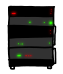
\includegraphics[width=\textwidth]{images/server.png}
        \end{column}
    \end{columns}
    
    \bigskip
    \bigskip
    (Images: \url{https://xkcd.com/1354/})
\end{frame}


\begin{frame}[fragile]
    \frametitle{Example (2): An \red{Insecure} Keyserver}

    \begin{columns}[b]
        \begin{column}{1.5cm}
        
\includegraphics[width=\textwidth]{images/meg.png}
        \end{column}

        \begin{column}{7cm}
\begin{tikzpicture}
\draw[->,very thick] (0,3) -- node[above]{upload $k = \Key{\id_1,\id_2}{\blob}$} (7,3);
\draw[->,very thick] (0,2) -- node[above]{confirm $\id_1 \mapsto k$} (7,2);
\draw[->,very thick] (0,1) -- node[above]{lookup $\id_1$} (7,1);
\draw[<-,very thick] (0,0) -- node[above]{result $\Key{\green{\id_1},\red{\id_2}}{\blob}$ \No} (7,0);
\end{tikzpicture}
        \end{column}

        \begin{column}{2cm}
        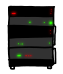
\includegraphics[width=\textwidth]{images/server.png}
        \end{column}
    \end{columns}
    
    \bigskip
    \bigskip
    (Images: \url{https://xkcd.com/1354/})
\end{frame}

\begin{frame}[fragile]
    \frametitle{Example (3): An \red{Insecure} Keyserver}

    \begin{columns}[b]
        \begin{column}{1.5cm}
        
\includegraphics[width=\textwidth]{images/meg.png}
        \end{column}

        \begin{column}{7cm}
\begin{tikzpicture}
\draw[->,very thick] (0,3) -- node[above]{upload $k = \Key{\id_1,\id_2}{\blob}$} (7,3);
\draw[->,very thick] (0,2) -- node[above]{confirm $\id_1 \mapsto k$} (7,2);
\draw[->,very thick] (0,1) -- node[above]{lookup $\blue{\fingerprint(k)}$} (7,1);
\draw[<-,very thick] (0,0) -- node[above]{result $\Key{\green{\id_1},\red{\id_2}}{\blob}$ \No} (7,0);
\end{tikzpicture}
        \end{column}

        \begin{column}{2cm}
        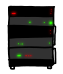
\includegraphics[width=\textwidth]{images/server.png}
        \end{column}
    \end{columns}
    
    \bigskip
    \bigskip
    (Images: \url{https://xkcd.com/1354/})
\end{frame}

\begin{frame}
    \frametitle{Goals \& Approach}
    \begin{itemize}
    \item Model actual Hagrid interface (tokens, emails, \ldots) \\
        \begin{itemize}
        \item detailed enough to capture the presented example
        \item models in \code{Scala} (abstract but executable)
        \end{itemize}
    \item Challenge: specify and check information flow security
        \begin{itemize}
        \item confirmation: \tabto{2.3cm} \emph{declassification}  \tabto{5.0cm} private $\rightsquigarrow$ public
        \item revocation:   \tabto{2.3cm} \emph{re-classification} \tabto{5.0cm} public  $\rightsquigarrow$ private
        \end{itemize}
    \item Focus on property-based \emph{testing} (\code{ScalaCheck})
    \end{itemize}

\medskip\pause

    \begin{itemize}
    \item[\No] Initial idea: test noninterference directly (two executions)
    \item[\Yes] Way too complex! Now much simpler approach
    \end{itemize}
\end{frame}

\begin{frame}[fragile]
    \frametitle{Central Ideas}

    Track finite \emph{histories} of events
    \begin{itemize}
    \item upload  \tabto{1.5cm} $k$
    \item confirm \tabto{1.5cm} $\id \mapsto \fingerprint(k)$
    \item revoke  \tabto{1.5cm} $\id \mapsto \fingerprint(k)$
    \end{itemize}
    $\to$ sufficient to specify which associations are \green{valid} at a time
    \bigskip\pause

    Stateful ``user''-actor executes a given history on server model
    \begin{itemize}
    \item keeps track of own key, identities, tokens
    \item keys and identities drawn randomly from some \blue{fixed sets}
    \end{itemize}
    \bigskip\pause
    
    ``Adversary'' calls server operations \code{byFingerprint}/\code{byEmail}
    \begin{itemize}
    \item compare results to \green{valid} associations
    \item for all \blue{possible} identities/keys
    \end{itemize}
\end{frame}

\begin{frame}
    \frametitle{Perspectives}
    Achieved so far
    \begin{itemize}
    \item Faithful executable model of Hagrid
    \item Property-directed security testing approach
    \item Random generators via \code{ScalaCheck}
    \end{itemize}
    \bigskip\pause

    Ongoing Work: Test Hagrid
    \begin{itemize}
    \item functional equivalence to model
    \item information flow security (directly)
    \end{itemize}
    Engineering effort: HTTP API, PGP keys, catch e-mails
\end{frame}

\begin{frame}
    \frametitle{Related Work}
    \begin{itemize}
    \item Model Checking Security Protocols (not on code)
    \item Testing noninterference quickly \\
          ~[Hriţcu et al; ICFP 2013] (instrumented execution)
    \item Semantic foundations based on attacker knowledge \\
          ~[Chudnov, Naumann; S\&P 2018] (no revocation)
    \end{itemize}
\end{frame}

\end{document}
